
\section{Research Plan}
\label{sec:research-plan}
%include a plan for validation of the research by experimentation and prototyping;

\begin{figure*}[thpb]
      \centering
      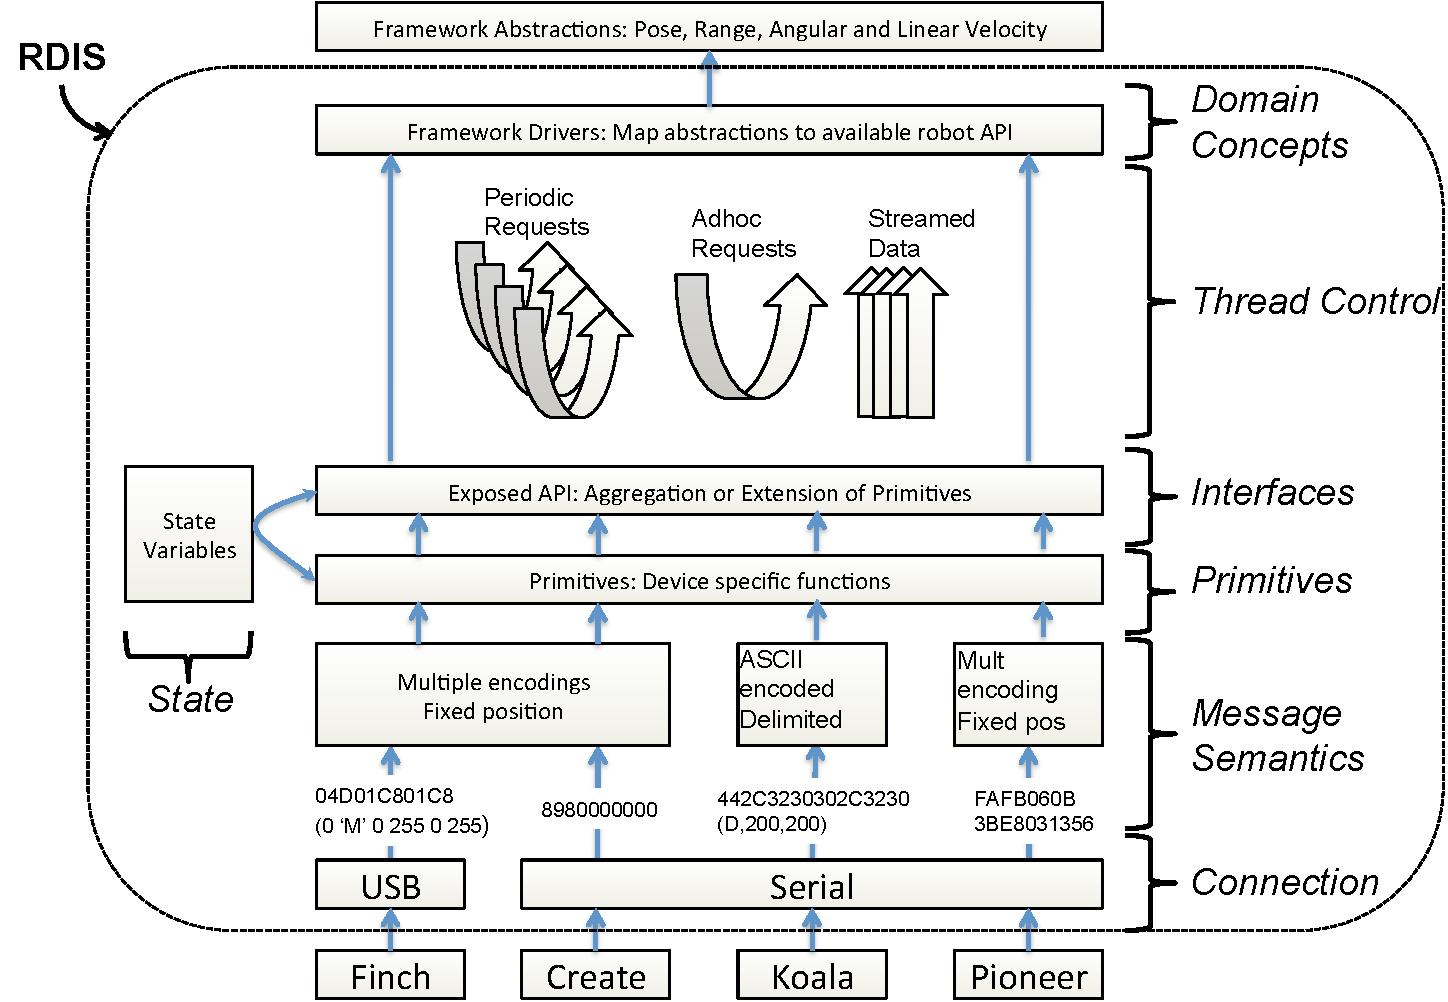
\includegraphics[width=5in]{dm.pdf}
      \caption{Preliminary domain model for mapping devices to frameworks.}
      \label{dm}
\end{figure*}

This preliminary result supports the idea that general robot devices can be described declaratively in a manner that supports discovery and that links to the backend processes.  The RDIS must be expanded to be useful in a larger context.  The work proposed as part of this effort will accomplish the following major innovations to RDIS as a contribution to the engineering of cyber-physical systems: 
\begin{enumerate}
\item Extend the processing models to include a larger set of execution semantics, 
\item Extend the actuation model to include a larger set of popular kinematic chains from both manufacturing and exploration robotics, and
\item Using RDIS as a hardware discovery mechanism, show composition of devices into a controller that is error-aware.   
\end{enumerate}

\subsection{Expansion of execution semantics}

The ability to generalize device to framework mapping requires documenting the concepts in existing mappings.  The domain model captures the invariant features of the device to framework mapping drives the contents of RDIS.  In Figure \ref{dm}, the domain is broken into seven related concepts: 1) connections, 2) state, 3) message semantics, 4) primitives, 5) interfaces, 6) thread control, and 7) robotics domain concepts.  {\sc Connection} refers to the transport used to communicate from the device driver to the framework.  Information needed to establish and maintain the connection is defined within this concept. The {\sc State} definition serves two purposes: 1) define constants relevant to other sections and 2) allow for state to be saved and retrieved as part of adhoc and periodic requests.   The {\sc Message Semantics} refers to the structure of the data which is actually sent to the robot over the connection. This specification is decided by the manufacturer and is generally uniform between primitives.   {\sc Primitives} focuses on describing the firmware interface in order to document the invariant features of the device.   The {\sc Interface} declaration, acting as a logical view of the {\sc Primitives},  specifies functions that are available to a developer to control a robot.   {\sc Domain Concepts} map interfaces to domain specific concepts in a framework agnostic manner.  These concepts are discussed in detail in \cite{Anderson2012}.

\begin{figure*}[thpb]
      \centering
      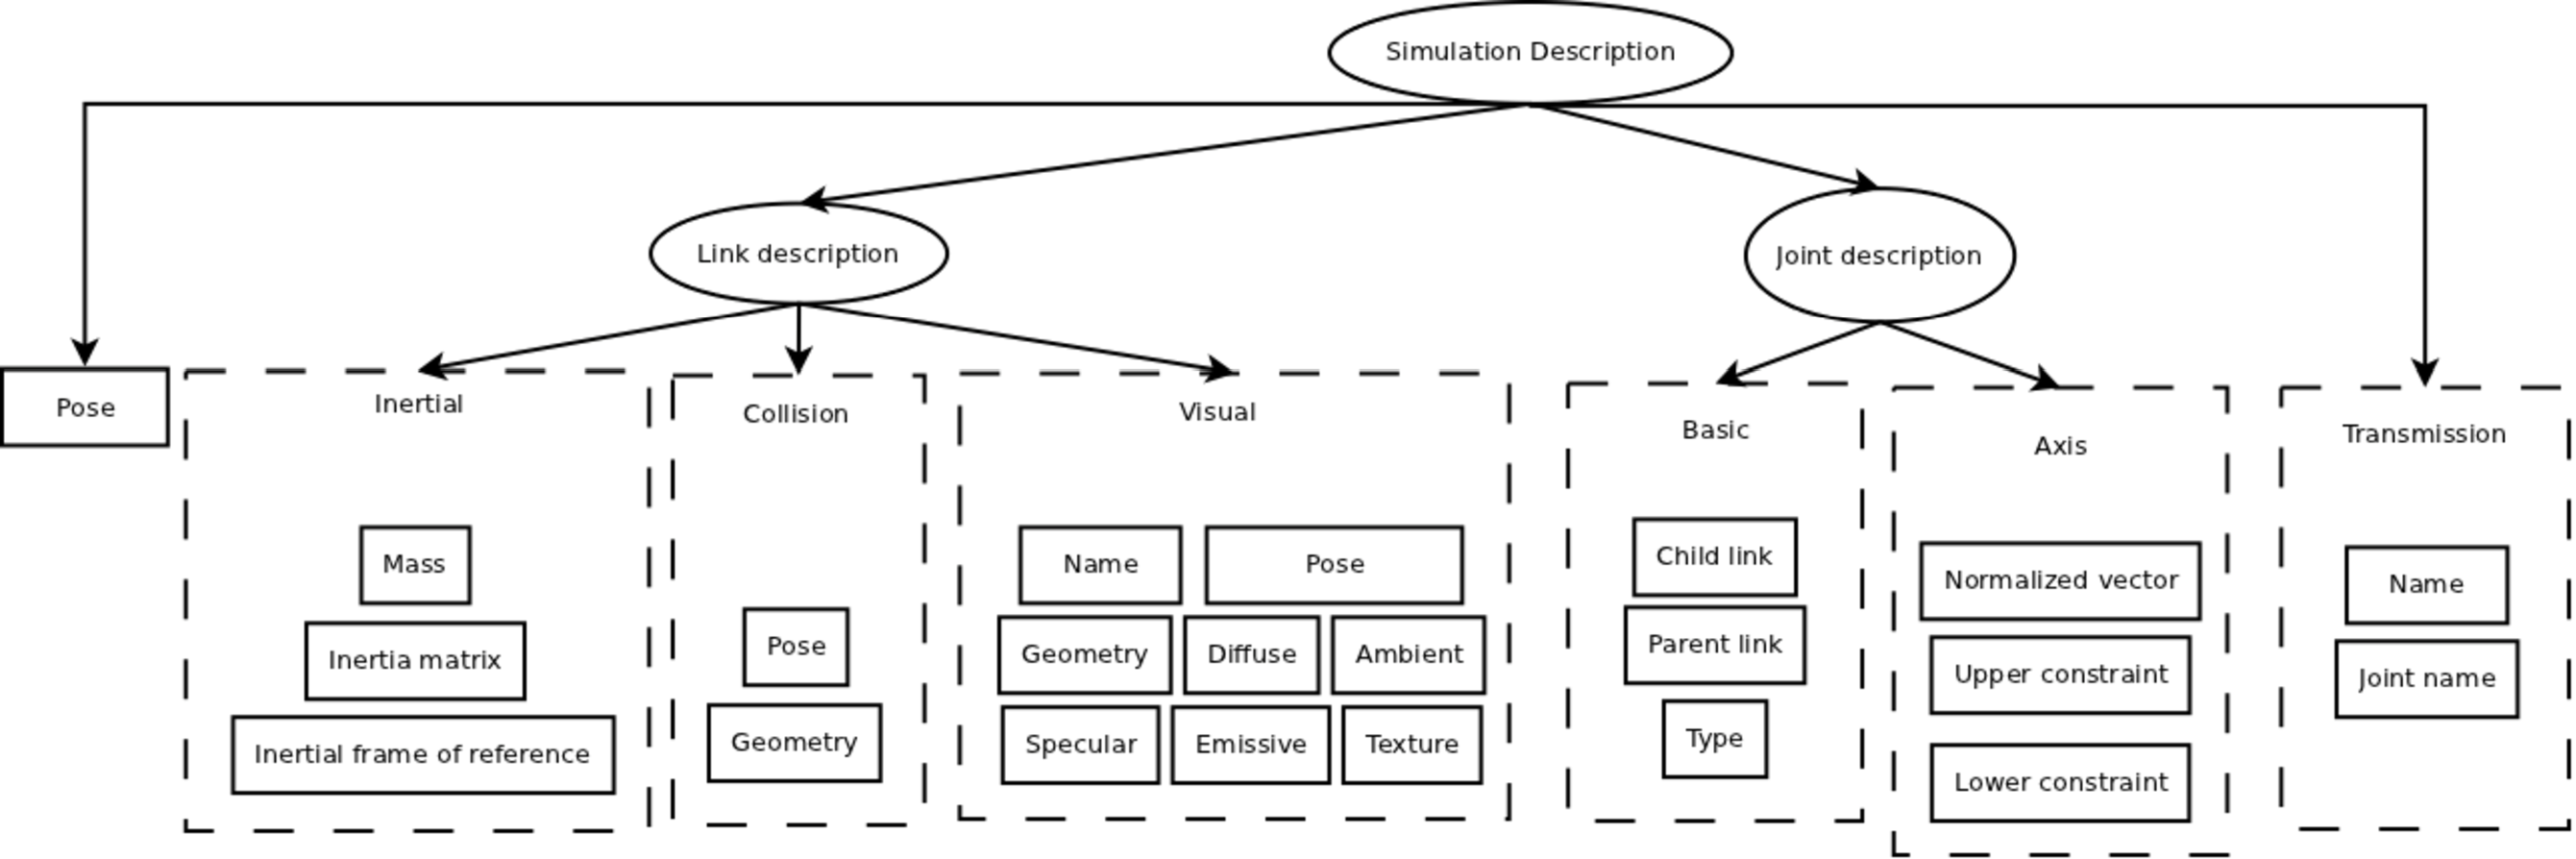
\includegraphics[width=6in]{kvc.pdf}
      \caption{General model for describing kinematics, appearance, collision and dynamics parameters sufficient for simulation on any simulation platform.  Currently targeted platforms include Gazebo, Webots, and ROS.}
      \label{kvc}
\end{figure*}

%These changes require updates to the specification and the underlying set of generation and utilizing tools. 

In this research, we expand the basic implementation of each concept to accommodate a larger set of embedded firmware controllers.  These tasks include: 
\begin{enumerate}
\item Addition of a complete kinematic, visual and collision description consistent with existing simulators and frameworks (see Figure \ref{kvc}).  Although initial focus will be upon the initial kinematic design (differential drive), the proposed model is designed to accommodate other kinematic designs.
\item Standard mechanism for error handling and notification at both the communication and primitive levels.  Error handling examples include re-establishment of connection or actions to take based on output parameters.  This is particularly relevant to platforms that require a heartbeat request periodically.
\item Expansion of the initial single-threaded implementation to include dual and multi-threading models.  A dual model accommodates different input and output threads while a multithreaded model support different frequencies for periodically submitted requests. 
\item Refinement of the state concept and how it matches to primitives and interfaces would provide a scripting language for transformation of data.  The state variable concept is instrumental in implementing periodic requests asynchronously from the client request/reply system.
\item Management of sensor and actuator error models consistent with existing frameworks will allow for manufacturer provided error models to be propagated to the framework or controller.  An example would be a transformation of encoder error to pose error.  Although all sources of error (systematic and non-systematic cannot be accounted for in this approach, it is currently better than existing approaches that abstract out specific device errors.
\end{enumerate}


\subsection{Expansion of domain concepts to additional kinematic chains}
Domain concepts map interfaces to domain specific concepts in a framework agnostic manner.  Each framework has a notion of a general set of abstract data types generated from device drivers such as pose estimates, pose relative to an identified landmark, control via linear and angular velocity along a dimension or axis, and point and fields of open distance.  The {\sc Domain concepts} definition identifies interfaces that map to the abstract concepts allowing for templates to map the abstract concepts to the existing interfaces available on a device.  

The initial scope of this research focuses on a set of domain concepts that represent popular platforms and devices and therefore are present in most frameworks as an abstraction.   The current set of domain concepts include {\sc differential drive} and {\sc range}.   Differential drive robots (robots with two opposing wheels on a single axis) are controllable using linear and rotational velocity.   Some frameworks explicitly recognize differential drive as a kinematic design (Player) while others group all platforms under a single fully expressive interface where the user must know which dimensions are controllable.  Acknowledging differential drive explicitly allows for an easier parameterization through state variables that denote odometry resolution, wheel size, offset of axis and wheel base.  For example, within the ROS system, a {\sc Twist} message type is used to provide control commands to a differential driver robot through linear and angular velocity.  Mapping the {\sc Twist} message to the Koala setMotor interface involves calculating left and right velocity from linear and angular velocity and calling the setMotor interface.  We map the differential drive domain concept to the {\sc setSpeed} interface (defined in the interface section.   {\sc transvel} and {\sc rotvel} are parameters of the controlDIfferentialDrive abstraction that map to the interface parameters.  The unit conversion (based on wheel base and encoder resolution) occurs between the interface and primitive to avoid having to encode the conversion multiple times.  Once an interface is designated as fulfilling a domain concept, the mapping better the interface and the framework specific mechanism can be generated.  The ROS template (discussed in more detail in \cite{Anderson2012}) maps each domain concept to the appropriate programming paradigm, which in this case is a subscription to the {\sc Twist} message and a callback handler that contains the code to map the {\sc Twist} message parameters to the interface parameters.   

RDIS will be updated to include additional sensors and kinematic chains.  Specifically, the {\sc range} will be extended to additional dimensions( {\sc range array}, and {\sc point cloud}) to represent ranges of open space in two and three dimensions.  These domain concepts relate to a set of readily available sensors including infrared, laser and ultrasonic range finders.   In addition, we can represent newer low-cost, 2D ranging sensors like the Microsoft Kinect.   Additional kinematic designs are motivated by partnerships with NASA and RTP.  NASA is migrating a robotic platform from VxWorks to Ubuntu with a future update to include RTLinux.  This custom kinematic chain involves manipulators with haptic sensors on a MLVDS bus (a new transport).  RTP (Huntsville Research Technology Park) is an initiative to by the governor of Alabama to create a National Robotics Technology Development and Training Center at Calhoun Community College.  Many robot platforms have been purchased and donated for training and are available for evaluation as candidate platforms for RDIS inclusion.  Both opportunities expands the platforms that can modeled and contribute to the domain model that can be generalized across other platforms. 

\subsection{RDIS as a component wrapper an discovery mechanism}
{\bf talk about how we can use rids to assist with development of controller by using existing tools for domain modeling}


\section{Project methodology, management, and dissemination plan}
\subsection{Team Member Roles, Responsibilities and Expertise}
%describe the roles, responsibilities, and expertise of the team members, how they cover the set of skills needed to realize the project goals and how their interactions will contribute to integration across core CPS disciplinary areas;

{\bf need something here about how a domain modeler is important to this research and what tools and expertise is helpful}

The success of the proposed research requires both breadth and depth in robotics hardware and software.  The PIs main research area centers on distributed robot systems.  However, her twelve years as a software engineer (culminating in a IT Architect position at IBM) has made the shortcomings of existing tools apparent.  She designed the circuit board and the software for the eROSI, a novel robot platform [46].  This platform featured an ASCII message-based API available via Bluetooth and images were served wirelessly via UHF channels.  These choices directly affected the platform usability for research students such as the undergraduate team at Berea College [47].  In addition, the PI has either programmed or modified drivers or firmware for robots and devices including the Koala, Finch, Create, Ar.Drone, Lego Mindstorms, Calliope (Dynamixel-based 4 DOF arm), Handyboard, GPS modules, lasers, analog and digital IR and ultrasonic sensors, and custom boards using ATMega chip and serial Bluetooth ICs to interface with Player/Stage, Alice/PREOP, ROS, Carmen, Webots and custom firmware applications.  In addition, the PI has studied open source implementations of other drivers and frameworks including PSOS (Pioneer robots), Tekkotsu, and LCM.  She was the organizer of the 2010 AAAI Robotics Workshop titled ``Enabling Intelligence through Middleware'' an effort to increase awareness of tools within the community and tool needs outside the community \cite{Croxell2008}. The PI is in a unique position given her expertise, experience and enthusiasm to affect accessibility of robotics controller development within the larger community.

\subsection{Dissemination Plan}
Broad dissemination plans include both the academic and non-academic communities.  Traditional academic dissemination plans include publications and conference presentations in both the educational and robotics software engineering communities.  Future plans include workshops at conference venues as well as at partner campuses will provide hands-on opportunities for those that wish to use the tool for teaching or design.  A website will be maintained and all software will be open source.  However, primary means of dissemination will utilize partnerships with manufacturers or tool developers as we have seen this method is effective at making hardware widely available.  The PI will also hold hands-on workshops both to inform and to gather feedback from the community.  

\subsection{Methodology}
The research approach consists of iterative design and integrated usability checks.  Rather than attempt to create the research tools in a single iteration, it is better to start with a core of features and iteratively add to those features. This approach allows for the usability testing within the first 18 months as an input into the next iteration.  The schedule details the work for two graduate students for the first three years: one student to focus on grammars and templates and one student to focus on RDSWare and usability testing.  Undergraduate students will assist with coding, testing and support activities.  The project team will meet weekly to discuss progress on features and use cases and any design issues.  Ongoing activities include dissemination through web sites, conferences and site visits.  